% Elsevier PREPRINT build (single column, 12pt). THIS is the submission
% manuscript; supplementary.tex resolves its cross-references against it.
%
% It started as a layout-only derivation of main2.tex (the 5p build) but has
% since been condensed for journal length: the two fidelity tables are merged,
% Problem Formulation is folded into the methods section, and the ablation,
% statistical and reproducibility detail is deferred to the supplement. Every
% number kept here is unchanged. main2.tex is no longer a source for this file;
% the two must be edited independently.
\documentclass[preprint,12pt]{elsarticle}
\usepackage[T1]{fontenc}
\usepackage[utf8]{inputenc}
\usepackage{lmodern}
\usepackage{amsmath}
\usepackage{amsfonts}
\usepackage{amssymb}
\usepackage{graphicx}
\usepackage{float}
\usepackage{placeins}
\usepackage{booktabs}
\usepackage{array}
\usepackage{adjustbox}
\usepackage{url}
\usepackage{xcolor}
\usepackage{tikz}
\usepackage{pdflscape}
\usepackage{microtype}
\usepackage{flafter}       % a float never appears before its first reference
% stfloats and the \dbl... fractions are two-column only; not needed here.
% Loosen float placement so wide floats settle near their reference instead of drifting.
\setcounter{topnumber}{3}
\setcounter{totalnumber}{5}
\renewcommand{\topfraction}{0.92}
\renewcommand{\textfraction}{0.07}
\renewcommand{\floatpagefraction}{0.72}
\usetikzlibrary{positioning,arrows.meta,shapes.geometric,fit,backgrounds,calc}
% --- Workflow-overview figure palette (mirrors the Mermaid version in doc/workflow_overview.md) ---
\definecolor{wfIndigo}{HTML}{312E81}
\definecolor{wfIndigoLight}{HTML}{E0E7FF}
\definecolor{wfIndigoMid}{HTML}{4F46E5}
\definecolor{wfAmberDark}{HTML}{D97706}
\definecolor{wfAmberLight}{HTML}{FEF3C7}
\definecolor{wfAmberText}{HTML}{78350F}
\definecolor{wfEmeraldDark}{HTML}{059669}
\definecolor{wfEmeraldLight}{HTML}{D1FAE5}
\definecolor{wfEmeraldText}{HTML}{064E3B}
\definecolor{wfEmeraldBg}{HTML}{ECFDF5}
\definecolor{wfPinkDark}{HTML}{DB2777}
\definecolor{wfPinkLight}{HTML}{FCE7F3}
\definecolor{wfPinkText}{HTML}{831843}
\definecolor{wfBlueDark}{HTML}{2563EB}
\definecolor{wfBlueLight}{HTML}{DBEAFE}
\definecolor{wfBlueText}{HTML}{1E3A8A}
\definecolor{wfBlueBg}{HTML}{EFF6FF}
\definecolor{wfViolet}{HTML}{7C3AED}
\definecolor{wfVioletDark}{HTML}{5B21B6}
\definecolor{wfRoseDark}{HTML}{E11D48}
\definecolor{wfRoseLight}{HTML}{FFE4E6}
\definecolor{wfRoseText}{HTML}{881337}
\definecolor{wfRoseBg}{HTML}{FFF1F2}
\definecolor{wfSlate}{HTML}{475569}
\newcolumntype{L}[1]{>{\raggedright\arraybackslash}p{#1}}

\newcommand{\widecomparisonplot}[1]{\includegraphics[width=0.76\textwidth]{#1}}

\newcommand{\encodingexampleplot}[1]{\includegraphics[width=0.42\linewidth]{#1}}
\newcommand{\subfigtext}[1]{\par\smallskip{\footnotesize #1\par}}
\setlength{\textfloatsep}{8pt plus 2pt minus 2pt}
\setlength{\floatsep}{8pt plus 2pt minus 2pt}
\setlength{\intextsep}{8pt plus 2pt minus 2pt}
\raggedbottom{}
% Single column at 12pt leaves fewer break points than the 5p build, so let TeX
% stretch a difficult paragraph rather than overflow the margin.
\setlength{\emergencystretch}{2em}
\hyphenation{op-tical net-works semi-conduc-tor}


\begin{document}

\begin{frontmatter}

\title{Controlled Reconstruction of Image-Based Time-Series Encodings: Operational Decoders for GAF, RP, and MTF Representations}

\author[mydass]{Adriano García-Giralda Milena}
\author[cls]{Francisco García Moreno}
\author[alg]{José Antonio Jiménez Madrid}
\author[cls]{María Bermúdez Edo}

\affiliation[mydass]{organization={MYDASS Research Group, University of Granada}, country={Spain}}
\affiliation[cls]{organization={Department of Computer Languages and Systems, University of Granada}, country={Spain}}
\affiliation[alg]{organization={Department of Algebra, University of Granada}, country={Spain}}







\begin{abstract}
Image-based time-series encodings expose temporal structure to image-domain models, but using them for signal generation or restoration requires the encoded image to map back to the time domain. We study this controlled reconstruction problem for Recurrence Plots (RP), Gramian Angular Summation and Difference Fields (GASF/GADF), and Markov Transition Fields (MTF), and contribute the two decoders the literature leaves open: a signed-RP decoder built on two-dimensional classical multidimensional scaling, adjacent-state overlap, and a closed-form orientation obtained from a $2\times2$ eigenproblem; and a restricted-branch GADF decoder with an image-derived boundary anchor and multi-pivot averaging. The GASF diagonal inverse is the established baseline, and MTF, being many-to-one, is evaluated only as a lossy control.

On 8,172 triaxial WISDM windows we assess fidelity, robustness, and downstream utility under one protocol. Every decoder recovers its normalised trajectory from the stored image alone, with no method-specific per-window metadata; returning to physical units uses a per-axis amplitude calibration shared by all four methods. RP, GASF, and GADF form a near-original tier, with mean absolute errors of 0.0142, 0.0205, and 0.0157\,m/s$^2$, and a native-operator ablation finds all three exact in floating point, so their clean round-trip error is attributable to 8-bit storage alone. Under a grouped subject-out protocol, simultaneous subject-cluster bootstrap intervals place all 18 RP/GASF/GADF classifier--method accuracy differences inside a one-percentage-point equivalence margin, whereas MTF meets it for none. The perturbation experiment measures local stability only: structurally imperfect and genuinely generated images remain unevaluated.
\end{abstract}

\begin{keyword}
Markov Transition Fields \sep Recurrence Plots \sep Gramian Angular Fields \sep Gramian Angular Difference Field \sep Time Series Reconstruction \sep Image Encoding \sep Machine Learning
\end{keyword}

\end{frontmatter}




\section{Introduction}\label{sec:introduction}
Image-based time-series representations such as recurrence plots (RP), Gramian angular fields (GAF) and Markov transition fields (MTF) turn a sequence into a matrix whose entries record a relationship between two temporal positions, so distances, angular relations and transition patterns become explicit spatial structure rather than relations a sequence model must infer from raw samples~\cite{wang2015encoding,wang2015encoding2}. Paired with an explicit inverse, they also offer an interface between time series and image-domain generative models~\cite{huang2023tsdigan,hellermann2026imagegan}.

Using them that way raises a question prior to classification accuracy: how much of the original waveform survives the round trip through the image? A synthetic or restored image is useful only if it maps back to a valid signal. This separates three concerns that are often discussed together: whether an image representation helps classification, whether a controlled image produced by a known encoder can be decoded, and whether a generative model can produce structurally valid images. This paper addresses the second, because only once it is settled can image-domain generation be evaluated meaningfully.

The setting is deliberately controlled. Every image evaluated here is the deterministic output of a known encoder and is stored as an 8-bit image. Each accelerometer axis is encoded independently, decoded in its normalised domain, and optionally returned to physical units using the same per-axis amplitude calibration. No diffusion model or GAN is trained, and we make no claim that arbitrary generated images are automatically physically valid.

Because the four operators retain different information, they lead to different reconstruction problems. GASF has a known diagonal inverse and serves as the invertible baseline. GADF contains angular differences but not absolute angles, so it requires a branch choice and an image-derived anchor. The continuous signed RP contains adjacent-state geometry, so decoding requires metric embedding, overlap alignment, and signed orientation selection. MTF discards within-state amplitudes and is inherently many-to-one, so its output is evaluated only as a representative trajectory. Figure~\ref{fig:workflow_overview} summarises the workflow, and Table~\ref{tab:decoder_contract} later states the decoder contract for each method.

The evaluation follows the same hierarchy for all methods: fidelity, robustness, and utility. Fidelity measures range-normalised pointwise error together with spectral shape and energy; robustness decodes perturbed and re-encoded images; and utility tests whether six original-trained classifiers retain subject-level accuracy within a one-percentage-point equivalence margin. These blocks answer three research questions:
\begin{itemize}
    \item \emph{(RQ1) fidelity}: does each decoder recover the signal from the image alone?
    \item \emph{(RQ2) stability}: how does the reconstruction degrade as the stored image is perturbed?
    \item \emph{(RQ3) equivalence}: is downstream subject-level accuracy equivalent to the original within a pre-set margin?
\end{itemize}
Both grouped trial-out and grouped subject-out three-fold splits are reported on the WISDM smartwatch accelerometer data.

The main contributions are:
\begin{itemize}
    \item \textbf{Signed-RP decoding:} an image-only decoder for continuous Lu--Tong recurrence plots of overlapping states, combining two-dimensional classical MDS, overlap consistency, and closed-form orientation recovery with signed selection, and requiring no per-window operator metadata.
    \item \textbf{GADF decoding:} a closed-form restricted-branch decoder whose image-derived boundary anchor and multi-pivot reconstruction make the normalised inverse operational, again without method-specific per-window metadata.
    \item \textbf{Controlled comparison:} a common protocol placing the new RP and GADF decoders beside the prior-art GASF diagonal inverse and a Fiedler-vector MTF representative, with MTF explicitly treated as a lossy control.
    \item \textbf{Validation framework:} an evaluation over fidelity, robustness, and utility, with range-normalised local-change and spectral errors, a repeated local perturbation test, and simultaneous subject-cluster equivalence intervals.
\end{itemize}

\begin{figure}[H]
\centering
% The workflow diagram was laid out for a full two-column width; scale it to the
% single-column text block of this build.
\resizebox{\textwidth}{!}{%
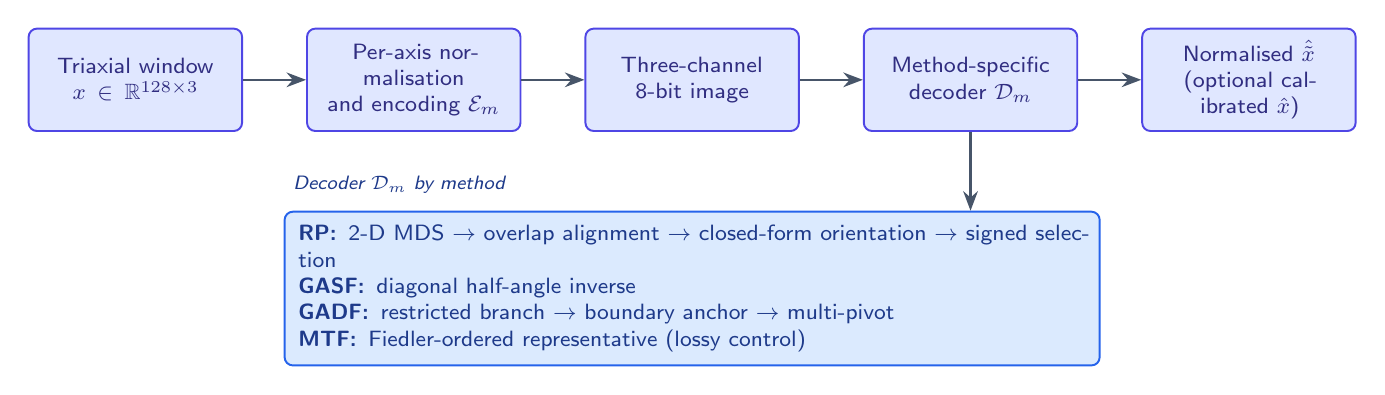
\begin{tikzpicture}[
  font=\sffamily\footnotesize,
  node distance=8mm,
  box/.style={rectangle, rounded corners=3pt, draw=wfIndigoMid, line width=0.7pt,
              fill=wfIndigoLight, text=wfIndigo, align=center,
              minimum height=13mm, text width=2.5cm, inner sep=3pt},
  detail/.style={rectangle, rounded corners=3pt, draw=wfBlueDark, line width=0.7pt,
                 fill=wfBlueLight, text=wfBlueText, align=left,
                 minimum height=9mm, text width=10cm, inner sep=5pt},
  dlabel/.style={text=wfBlueText, font=\sffamily\scriptsize\itshape},
  arrow/.style={->, draw=wfSlate, line width=0.9pt, >=Stealth}
]
  \node[box] (input) {Triaxial window\\$x\in\mathbb{R}^{128\times3}$};
  \node[box, right=of input] (encode) {Per-axis normalisation\\and encoding $\mathcal E_m$};
  \node[box, right=of encode] (image) {Three-channel\\8-bit image};
  \node[box, right=of image] (decode) {Method-specific\\decoder $\mathcal D_m$};
  \node[box, right=of decode] (output) {Normalised $\hat{\tilde x}$\\(optional calibrated $\hat x$)};
  \draw[arrow] (input) -- (encode);
  \draw[arrow] (encode) -- (image);
  \draw[arrow] (image) -- (decode);
  \draw[arrow] (decode) -- (output);

  \node[detail, below=10mm of image] (methods) {%
    \textbf{RP:}\enspace 2-D MDS $\to$ overlap alignment $\to$ closed-form orientation $\to$ signed selection\\
    \textbf{GASF:}\enspace diagonal half-angle inverse\\
    \textbf{GADF:}\enspace restricted branch $\to$ boundary anchor $\to$ multi-pivot\\
    \textbf{MTF:}\enspace Fiedler-ordered representative (lossy control)};
  \node[dlabel, above=1mm of methods.north west, anchor=south west] {Decoder $\mathcal D_m$ by method};
  \draw[arrow] (decode.south) -- (decode.south |- methods.north);
\end{tikzpicture}}
\caption{Controlled reconstruction workflow. Each axis is normalised, encoded, and stored as an 8-bit image channel, then decoded in its method-specific normalised domain and optionally returned to physical units with per-axis calibration. The lower box expands the method-specific decoder $\mathcal D_m$.}\label{fig:workflow_overview}
\end{figure}

\section{Background and Related Work}\label{sec:related_encodings}

\subsection{Time-series imaging}
Time-series imaging compares many temporal positions at once: rows and columns preserve the order of the window, and each pixel stores a method-specific relationship between the two positions it indexes, so a single frame exposes distances, periodicities, and symmetries as spatial structure. Wang and Oates introduced GAF and MTF images for classification and imputation with convolutional networks~\cite{wang2015encoding,wang2015encoding2}; recurrence plots predate that line as a tool for visualising when a dynamical system returns to a previously visited region of its state space~\cite{eckmann1987recurrence,marwan2007recurrence}, and were later adopted as image inputs for the same reason. The family has been applied to human activity recognition from inertial signals~\cite{ahmad2021inertial}, to multivariate anomaly detection~\cite{ma2024anomaly}, and to missing-value imputation~\cite{huamin2020reconstruction}, and more recently as the substrate for image-domain generative models that invert back to the temporal domain, such as GASF-based traffic imputation~\cite{huang2023tsdigan} and the XIRP representation designed for GAN generation followed by inversion~\cite{hellermann2026imagegan}.

These applications establish that two-dimensional encodings are useful inputs for discriminative and generative models. They do not establish that the original waveform is preserved: a representation can predict an activity label while discarding the amplitude, phase, or ordering information that reconstruction requires. The rest of this section therefore asks what information each operator retains, and what decoding work already exists.


\begin{figure}[H]
\centering
\begin{minipage}[t]{0.24\linewidth}
\centering
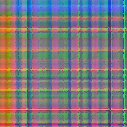
\includegraphics[width=\linewidth]{images/1600xtrp0.png}
\subfigtext{(a) RP}
\end{minipage}\hfill
\begin{minipage}[t]{0.24\linewidth}
\centering
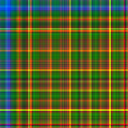
\includegraphics[width=\linewidth]{images/1600x0tgasf.png} % chktex 29
\subfigtext{(b) GASF}
\end{minipage}\hfill
\begin{minipage}[t]{0.24\linewidth}
\centering
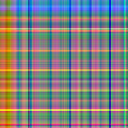
\includegraphics[width=\linewidth]{images/1600x0tgadf.png} % chktex 29
\subfigtext{(c) GADF}
\end{minipage}\hfill
\begin{minipage}[t]{0.24\linewidth}
\centering
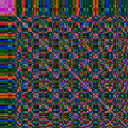
\includegraphics[width=\linewidth]{images/1600x0tmtf.png} % chktex 29
\subfigtext{(d) MTF}
\end{minipage}
\caption{RP, GASF, GADF, and MTF encodings of the same triaxial WISDM walking window, with the $x,y,z$ axes mapped to the RGB channels. RP is $127\times127$ because of the adjacent-state embedding; the other three are $128\times128$.}\label{fig:encodings_main}
\end{figure}

\subsection{Encoding methods}
\label{sec:encoding_methods}

Figure~\ref{fig:encodings_main} shows the four encodings of a single WISDM window, where the symmetry of GASF, the antisymmetry of GADF, and the discrete transition-level regions of MTF are already visible. This subsection defines the operators that produce them; previously proposed reconstruction approaches are reviewed in Section~\ref{sec:prior_reconstruction}.

\subsubsection{Recurrence plots}
\label{sec:rp_encoding}

Following delay-coordinate embedding~\cite{takens1981detecting}, a scalar sequence \(x=(x_1,\ldots,x_N)\) is represented by the overlapping states
\[
s_i=(x_i,x_{i+1})\in\mathbb{R}^2,
\qquad i=1,\ldots,N-1.
\]
A conventional recurrence plot is constructed from pairwise distances between these states, often after applying a recurrence threshold~\cite{eckmann1987recurrence,marwan2007recurrence}. Such unsigned distance representations describe state proximity but do not retain the direction of the corresponding displacement.

For the present study, we adopt the continuous signed construction proposed by Lu and Tong~\cite{lu2019robust}. Given the reference direction
\[
v=\frac{[1,1]^\top}{\sqrt{2}},
\]
the recurrence matrix is defined as
\begin{equation}
R_{ij}=\sigma(i,j)\lVert s_i-s_j\rVert_2,
\label{eq:FormulaRP}
\end{equation}
where, for \(\lVert s_i-s_j\rVert_2>0\),
\[
\hat u_{ij}=\frac{s_i-s_j}{\lVert s_i-s_j\rVert_2},
\]
and
\begin{equation}
\sigma(i,j)=
\begin{cases}
1,
&
\lVert s_i-s_j\rVert_2=0
\ \text{or}
\hat u_{ij}\cdot v\geq\cos(\pi/4),
\\
-1,
&
\text{otherwise}.
\end{cases}
\end{equation}

The magnitude of \(R_{ij}\) holds the pairwise Euclidean geometry of the adjacent states and its sign a directional distinction relative to \(v\). Because the \(N-1\) states share samples, that geometry also carries a sequential consistency absent from a generic point cloud, which the decoder of Section~\ref{sec:rp_reconstruction_method} exploits.

\subsubsection{Gramian angular fields}
\label{sec:gaf_encoding}

After normalisation to the method-specific interval, each sample is mapped to an angular coordinate,
\[
\phi_i=\arccos(\tilde{x}_i).
\]
Gramian Angular Summation Fields (GASF) and Gramian Angular Difference Fields (GADF) are then defined as~\cite{wang2015encoding}
\begin{align}
G^{\mathrm{S}}_{ij}
&=\cos(\phi_i+\phi_j) \nonumber\\
&=\tilde{x}_i\tilde{x}_j
-\sqrt{1-\tilde{x}_i^2}\sqrt{1-\tilde{x}_j^2},
\label{eq:gasf_indexed}
\\
G^{\mathrm{D}}_{ij}
&=\sin(\phi_i-\phi_j) \nonumber\\
&=\sqrt{1-\tilde{x}_i^2}\tilde{x}_j
-\tilde{x}_i\sqrt{1-\tilde{x}_j^2}.
\label{eq:gadf_indexed}
\end{align}

The two fields retain different information. GASF is symmetric and its diagonal, \(G^{\mathrm{S}}_{ii}=\cos(2\phi_i)\), carries a single-sample angular term. GADF is antisymmetric with an identically zero diagonal, \(G^{\mathrm{D}}_{ii}=0\), so it represents relative angular differences and their direction but never the absolute angular position of a sample. Any GADF inverse must therefore resolve both the ambiguity of the inverse sine and the global angular offset the difference operator removes.

\subsubsection{Markov transition fields}
\label{sec:mtf_definition}

MTF first assigns every sample \(x_t\) to one of \(Q\) quantile states \(q_t\)~\cite{wang2015encoding}. A first-order transition matrix is then estimated as
\[
W_{p,q}=P(q_{t+1}=q\mid q_t=p),
\]
where \(W_{p,q}\) represents the probability of moving from state \(p\) to state \(q\).

The transition matrix is expanded over the original temporal grid according to
\[
M_{a,b}=W_{q_a,q_b},
\qquad
a,b=1,\ldots,N.
\]
so each image entry is the transition probability between the quantile states occupied at two temporal positions.

MTF thus retains state membership and transition structure but not a sample's amplitude within its quantile interval: samples in the same state share a transition profile, and the numerical ordering of the latent states is not identifiable from the image values alone. The mapping is inherently many-to-one.

\subsection{Prior reconstruction methods}
\label{sec:prior_reconstruction}

Reconstruction is specific to the information each encoding retains. The literature provides a direct inverse for GASF and geometric reconstruction methods for earlier recurrence plots, whereas GADF and MTF require different treatment.

\subsubsection{Recurrence plots}

Earlier RP reconstruction follows two main routes. Hirata et al.\ start from a thresholded recurrence plot, convert it into a weighted graph, estimate distances along graph paths, and apply multidimensional scaling (MDS) to reproduce the topological shape of the original trajectory~\cite{hirata2008reproduction}. Sipers et al.\ instead study unthresholded recurrence plots generated by time-delay embeddings. They characterise when the underlying scalar signal is identifiable up to its mean and a choice of sign, and introduce a distance between recurrence plots that supports reconstruction by minimisation~\cite{sipers2011unique}. Their later method uses a singular-value decomposition for reconstruction under disturbances and extends the analysis to multi-level recurrence plots, which preserve more information than binary plots while remaining compressed~\cite{sipers2017robust}.

These studies establish that unsigned recurrence information can support geometric or signal reconstruction, but none is a direct decoder for the continuous signed adjacent-state operator in Equation~\ref{eq:FormulaRP}. Here, \(\lvert R\rvert\) already supplies the dense Euclidean distances between two-dimensional states, so no graph-distance approximation is needed. The remaining problem is different: MDS recovers the state configuration only up to an orthogonal transformation, and the scalar sequence must then be obtained by enforcing the shared-sample relation between consecutive states. The Lu--Tong signs provide the additional directional information used to select the remaining orientation.

\subsubsection{Gramian angular fields}

For GASF, Wang and Oates give a direct inverse from the main diagonal. If the signal is normalised to \([0,1]\), then \(\phi_i\in[0,\pi/2]\) and
\[
\tilde{x}_i=\sqrt{\frac{G^{\mathrm{S}}_{ii}+1}{2}}.
\]
The non-negative square root is unique on this branch. Their imputation pipeline first restores a damaged GASF with a denoising autoencoder and then applies this diagonal inverse~\cite{wang2015encoding}. Tao et al.\ later use RP and GAF images with a denoising autoencoder to reconstruct missing time-series values~\cite{huamin2020reconstruction}. Both studies address missing-value imputation through learned image restoration; neither provides the signed-RP or GADF decoder required here.

GADF does not inherit that diagonal decoder because \(G^{\mathrm{D}}_{ii}=0\) for every sample. Wang and Oates state that GADF constructed from \([0,1]\)-scaled data has an accurate inverse map, but their operational imputation procedure and explicit inverse formula use GASF~\cite{wang2015encoding}. In particular, they do not specify a decoder that resolves the inverse-sine branch, restores the global angular offset removed by pairwise differences, and remains usable after finite-precision image storage. Those are the three issues addressed by the restricted-branch GADF decoder proposed in Section~\ref{sec:gadf_reconstruction_proposal}.

\subsubsection{Markov transition fields}

Wang and Oates report substantially greater uncertainty when reconstructing MTF than GAF and note that even approximate signal recovery is difficult~\cite{wang2015encoding}. This limitation follows directly from the operator: quantile assignment discards each sample's position within its bin, so different continuous signals can produce the same state sequence, transition matrix, and MTF image. The mapping is therefore many-to-one, and no image-only decoder can recover the exact original amplitudes without additional information. An MTF decoder can return only a representative trajectory compatible with the inferred quantised states; it should not be interpreted as an inverse.


\subsection{Research gap}\label{sec:research_gap}
Two gaps follow from this review. First, the reviewed literature does not provide an operational decoder for either restricted-branch GADF or the continuous signed adjacent-state RP considered here, particularly after finite-precision image storage. Second, it does not provide a controlled comparison of RP, GASF, GADF, and MTF under the same reconstruction, perturbation, and downstream-utility protocol. This work addresses both gaps: it proposes operational GADF and signed-RP decoders, requires no method-specific per-window metadata for normalised reconstruction, and evaluates all four methods together, with GASF as the established invertible baseline and MTF as a lossy control.

\section{Reconstruction Framework and Methods}\label{sec:proposed_methods}

\subsection{Problem setup and storage protocol}\label{sec:shared_protocol}

The formal problem is not to classify an image, but to test the round trip from a signal to an image and back to a signal. Let \(x=(x_1,\ldots,x_N)\) denote one axis of an accelerometer window. Method \(m\) applies a normaliser \(\mathcal N_m\), an encoder \(\mathcal E_m\), and a decoder \(\mathcal D_m\):
\[
\tilde x^{(m)}=\mathcal N_m(x),\qquad
M^{(m)}=\mathcal E_m(\tilde x^{(m)}),
\]
\[
\hat{\tilde x}^{(m)}=\mathcal D_m(M^{(m)}).
\]
Here \(M^{(m)}\in\mathbb R^{N_m\times N_m}\), with \(N_m=N\) for GASF, GADF, and MTF and \(N_m=N-1\) for the adjacent-state RP\@. The primary reconstruction problem is to recover the normalised signal \(\hat{\tilde x}^{(m)}\); returning to physical units,
\[
\hat x=\mathcal N_m^{-1}(\hat{\tilde x}^{(m)};x_{\min},x_{\max}),
\]
is a common optional calibration step. Each accelerometer axis is encoded independently, stored as one RGB channel, decoded, and regrouped into a triaxial window.

Encoded matrices are stored and reread as 8-bit PNG images. Every matrix is written with an affine per-window map onto \([0,255]\), and the GASF and GADF images are read back with the fixed operator range \([-1,1]\), so their inverse needs no per-window information. For GASF the two maps coincide exactly: normalising the signal to \([0,1]\) forces \(\phi\) to attain both \(0\) and \(\pi/2\), so the diagonal reaches \(+1\) and \(-1\) in every non-constant window. For GADF the attained extreme is instead \(\pm2\alpha\sqrt{1-\alpha^2}\), so reading the image as \([-1,1]\) applies a fixed gain of \(1/(2\alpha\sqrt{1-\alpha^2})\); at \(\alpha=0.7\) this is \(1.00013\), an endpoint discrepancy below one 8-bit intensity step. Our stored GADF matrices follow the transposed convention \(\sin(\phi_j-\phi_i)\), so an implementation working in the notation of Equation~\ref{eq:gadf_indexed} must negate the image it reads. MTF already occupies \([0,1]\) and is stored without renormalisation. RP keeps its per-window map, since its signed-distance range varies from window to window; the decoder removes the resulting per-window shift by centring on the zero-valued diagonal, leaving an unknown positive scale that classical MDS and the final range map absorb. Table~\ref{tab:decoder_contract} separates information required for normalised reconstruction from the optional amplitude calibration used for physical units.

\begin{table}[H]
\centering
\caption{Decoder outputs and the method-specific per-window information required under the current storage protocol. Fixed encoder conventions are assumed known.}\label{tab:decoder_contract}
\small
\setlength{\tabcolsep}{6pt}
\begin{tabular}{@{}L{0.12\textwidth}L{0.38\textwidth}L{0.40\textwidth}@{}}
\toprule
Method & Decoder output & Required per-window information \\
\midrule
RP   & Normalised waveform & None (zero level from the diagonal; residual positive scale immaterial) \\
GASF & Normalised waveform in $[0,1]$ & None \\
GADF & Normalised waveform in $[-\alpha,\alpha]$ & None \\
MTF  & Quantile-level representative trajectory & None \\
\bottomrule
\end{tabular}

\smallskip
\footnotesize
 Returning any decoded output to the observed signal scale additionally requires the common per-axis calibration $(x_{\min},x_{\max})$.
\end{table}

Normalised reconstruction is therefore image-only for all four methods under their stated contracts, and physical-unit recovery additionally uses the common per-axis calibration \((x_{\min},x_{\max})\). What fails is inverting the RP image with an incorrect external range, not the absence of the operator range itself; that comparison, and the GADF gain above, are quantified in the Supplementary Material.

\subsection{Signed recurrence-plot decoder}\label{sec:rp_reconstruction_method}

For the continuous signed RP in Equation~\ref{eq:FormulaRP}, the magnitude matrix contains Euclidean distances between adjacent states \(s_i=(x_i,x_{i+1})\). The proposed decoder recovers their full two-dimensional geometry and fixes the orthogonal ambiguity using overlap and sign:


\begin{enumerate}
\item Recover the signed matrix from the image without per-window metadata. The RP diagonal is identically zero, so its constant stored pixel level locates \(R=0\); subtracting the diagonal median, \(R^{\mathrm{obs}}=\mathrm{PNG}-\operatorname{median}_i\mathrm{PNG}_{ii}\), recovers the signed matrix up to a positive scale, which the classical-MDS step and the final range map absorb. Form the symmetric distance matrix
\[
D_{ij}=\tfrac12\bigl(|R^{\mathrm{obs}}_{ij}|+|R^{\mathrm{obs}}_{ji}|\bigr),\qquad D_{ii}=0.
\]
\item Apply classical MDS to \(D\)~\cite{Torgerson1952}. If \(J=I-\mathbf1\mathbf1^\top/(N-1)\), eigendecomposition of \(-\tfrac12JD^2J\) yields the two leading coordinates \(Y=V_2\Lambda_2^{1/2}\).

\item Fix the two-dimensional orthogonal transformation of \(Y\) in closed form. Every such transformation can be written \(Q_{\theta,\eta}=\mathrm{rot}(\theta)\,\mathrm{diag}(1,\eta)\), with rotation angle \(\theta\) and reflection parity \(\eta\in\{+1,-1\}\). Writing \(Z=YQ_{\theta,\eta}\) and reading the candidate states as \((a_i,b_i)=(Z_{i1},Z_{i2})\), the criterion is the adjacent-state overlap: \(b_i\) and \(a_{i+1}\) are two estimates of the same sample \(x_{i+1}\), so their disagreement measures the error of the orientation. Pairwise distances fix the configuration only up to a common translation \(\delta\) along the overlap direction, so the angle and that translation are chosen together,
\[
\min_{\theta,\delta}\;J,
\qquad
J=\sum_{i=1}^{N-2}{\bigl(b_i-a_{i+1}+\delta\bigr)}^2,
\]
the recovered offset being applied symmetrically as \(a_i\mapsto a_i-\delta/2\) and \(b_i\mapsto b_i+\delta/2\).

For fixed \(\eta\), the raw overlap residual is linear in \((\cos\theta,\sin\theta)\):
\[
b_i-a_{i+1}=A_i\cos\theta+B_i\sin\theta,
\quad
\begin{aligned}
A_i&=\eta Y_{i2}-Y_{i+1,1},\\
B_i&=-\eta Y_{i1}-Y_{i+1,2}.
\end{aligned}
\]
Hence for any \(\theta\) the optimal translation is the negated mean residual, \(\delta^\star=-\frac{1}{N-2}\sum_i(b_i-a_{i+1})\), and substituting it simply mean-centres the two coefficients. With \(\tilde A_i=A_i-\bar A\), \(\tilde B_i=B_i-\bar B\), and \(\tilde C=[\,\tilde A\;\;\tilde B\,]\in\mathbb R^{(N-2)\times2}\), the profiled objective is the quadratic form
\[
J\bigl(\theta,\delta^\star\bigr)=u^\top H_\eta u,
\qquad
H_\eta=\tilde C^\top\tilde C,
\qquad
u=\begin{bmatrix}\cos\theta\\ \sin\theta\end{bmatrix}.
\]
Because \(\lVert u\rVert=1\), minimising this Rayleigh quotient over the unit circle is an eigenproblem: the minimiser is the unit eigenvector of the symmetric \(2\times2\) matrix \(H_\eta\) belonging to its smaller eigenvalue. Both signs \(\pm u\) attain the same minimum, so the two parities give exactly four globally optimal candidates and no angular discretisation is required. Among them, select the orientation whose regenerated signed RP is closest to \(R^{\mathrm{obs}}\) in Frobenius norm, comparing both after normalisation to unit norm so the choice (and any tie among near-minimisers) is resolved independently of the unknown positive scale.
\item For aligned states \(\hat s_i=(a_i,b_i)\), recover all \(N\) samples:
\[
\begin{aligned}
\hat x_1 &= a_1,\\
\hat x_i &= \tfrac12(b_{i-1}+a_i),\quad 2\le i\le N-1,\\
\hat x_N &= b_{N-1}.
\end{aligned}
\]
\item Pairwise distances leave a common translation and a positive scale undetermined. Map the recovered sequence's minimum and maximum to the known normalised range to fix both; physical-unit recovery, if required, then uses the shared calibration.
\end{enumerate}

Retaining both MDS dimensions is essential because the embedded states are genuinely two-dimensional. The signed comparison resolves the reflection that remains after overlap alignment; Section~\ref{sec:decoder_ablation} summarises both choices.

Solving the orientation in closed form costs \(O(N)\), the cost of forming \(H_\eta\), instead of the \(O(n_\theta N)\) of an angular grid with \(n_\theta\) candidates, and it is exact rather than accurate to the grid spacing; the decoder as a whole remains dominated by the classical-MDS eigendecomposition, \(O(N^3)\). Measured timings at \(N=128\) are reported in the Supplementary Material, where the angular grid is retained as a historical baseline.

\subsection{GASF diagonal inverse}\label{sec:gasf_reconstruction_method}

GASF is the controlled prior-art baseline~\cite{wang2015encoding}. On the branch \(\phi_i\in[0,\pi/2]\),
\[
G^{\mathrm S}_{ii}=\cos(2\phi_i),\qquad
\hat\phi_i=\tfrac12\arccos(G^{\mathrm S}_{ii}),\qquad
\hat{\tilde x}_i=\cos(\hat\phi_i).
\]
The branch condition matters: under \([-1,1]\) scaling the diagonal determines only \(|\tilde x_i|\). With the \([0,1]\) protocol used here, the normalised shape follows from the diagonal and the amplitude range is needed only for optional physical-unit recovery.

\subsection{Restricted-branch GADF decoder}\label{sec:gadf_reconstruction_proposal}

GADF contains relative angles \(G^{\mathrm D}_{ij}=\sin(\phi_i-\phi_j)\) but no diagonal amplitude information. We scale each non-constant window to
\[
\bar x_t=2\alpha\frac{x_t-x_{\min}}{x_{\max}-x_{\min}}-\alpha,
\qquad \alpha=0.7,
\]
so \(\phi_t=\arccos(\bar x_t)\). A unique principal-branch inverse requires
\[
\max_{i,j}|\phi_i-\phi_j|
=\pi-2\arccos(\alpha)<\frac{\pi}{2},
\]
which is equivalent to \(\alpha<1/\sqrt2\). The choice \(\alpha=0.7\) is therefore close to the largest admissible symmetric range while retaining a numerical margin. Under this restriction,
\[
\arcsin(G^{\mathrm D}_{ij})=\phi_i-\phi_j.
\]

A pivot row \(p\) determines all angles relative to \(\phi_p\):

\[
\phi_j=\phi_p-\arcsin(G^{\mathrm D}_{pj}).
\]
The remaining global offset is fixed from the image. Per-window normalisation guarantees samples at both boundaries \(\pm\alpha\). Define
\(\bar C=N^{-1}\sum_j\cos\phi_j\) and \(\bar S=N^{-1}\sum_j\sin\phi_j\). The row mean
\[
\mu_i=\frac1N\sum_j G^{\mathrm D}_{ij}
=\bar C\sin\phi_i-\bar S\cos\phi_i
\]

is strictly increasing over the restricted angular interval. Indeed, writing
\(\bar C=R\cos\psi\) and \(\bar S=R\sin\psi\) gives
\(\mu(\phi)=R\sin(\phi-\psi)\). The mean direction \(\psi\) lies inside the cone
spanned by the sample angles; because that cone has width below \(\pi/2\),
\(\mu'(\phi)=R\cos(\phi-\psi)>0\) throughout the interval. Hence
\[
e=\arg\max_i|\mu_i|
\]
identifies a boundary row. Because \(\mu\) increases with \(\phi\), its sign resolves which boundary: \(\mu_e>0\) gives \(\phi_e=\arccos(-\alpha)\) and \(\mu_e<0\) gives \(\phi_e=\arccos(\alpha)\). For each of the \(n_p=5\) rows with the smallest \(|\mu_p|\),
\[
\begin{aligned}
\hat\phi^{(p)}_j
&=\phi_e-\arcsin(G^{\mathrm D}_{ep})-\arcsin(G^{\mathrm D}_{pj}),\\
\hat{\bar x}_j
&=\cos\left(\frac1{n_p}\sum_{p}\hat\phi^{(p)}_j\right).
\end{aligned}
\]
Averaging angles over central pivots reduces PNG quantisation noise without changing the \(O(N^2)\) cost of reading the matrix and computing its row means. The inverse is exact in real arithmetic under the branch, boundary, and sign assumptions; it is not a generic inverse for unconstrained GADF images.

\subsection{Best-effort Fiedler-vector MTF representative}\label{sec:mtf_reconstruction_method}

MTF is many-to-one, so its decoder returns not an inverse but a representative trajectory compatible with the transition structure. Equal rows of a clean MTF correspond to the same quantile state, so the decoder clusters the \(N\) rows into \(Q\) groups, estimates \(W\) by averaging image blocks, orders the recovered groups by the Fiedler vector of the Laplacian of its symmetrisation, following spectral seriation~\cite{Atkins1998}, and assigns the midpoint \((k-\tfrac12)/Q\) to samples in ordered group \(k\). The Fiedler coordinate supplies a one-dimensional ordering of the latent groups, which for a general transition graph is a heuristic rather than an identifiability guarantee.

Two ambiguities remain by construction: the image does not determine the global reversal of the amplitude order, and all values within a bin share one representative. We use \(Q=4\); the implementation, the bin-count sweep, and the metadata variants are in the Supplementary Material.
\section{Experimental Protocol}\label{sec:experimental_protocol}

\subsection{Dataset and segmentation}

We use the 20\,Hz smartwatch accelerometer stream of the WISDM Smartphone and Smartwatch Activity and Biometrics Dataset~\cite{misc_wisdm_smartphone_and_smartwatch_activity_and_biometrics_dataset__507}. Five nearly balanced activities are retained: standing (20.6\%), sitting (20.2\%), walking (20.0\%), stairs (19.7\%), and jogging (19.5\%). Within every contiguous subject--activity recording, we form non-overlapping windows of \(N=128\) samples (6.4\,s) and discard the final incomplete block. No window crosses a subject or activity boundary.

This produces 8,172 labelled triaxial windows from 51 subjects, or 24,516 one-axis reconstructions. GASF, GADF, and MTF images are \(128\times128\); the adjacent-state RP is \(127\times127\), and its overlap reconstruction returns 128 samples.

Two complementary three-fold protocols are evaluated, both class-stratified and both grouped so that no recording unit is split between train and test. The \emph{trial-out} split keeps every trial --- one subject performing one activity, 253 trials in total --- in a single fold, so adjacent windows of the same recording never straddle the split; a subject may still contribute other activities to training, so this protocol measures reconstruction-induced distribution shift within the observed population. The \emph{grouped subject-out} split keeps all windows of a subject in one fold, holding out complete individuals, and is our \emph{primary} protocol because it estimates generalisation to unseen people; the trial-out split is reported as a within-population reference. In either protocol the union of the three test folds is the same 8,172 windows, so pooled reconstruction errors are protocol-independent for these deterministic, untrained decoders; classifier performance differs because a new model is trained per fold. Fold composition and the full trial-out comparison are in the Supplementary Material.

\subsection{Evaluation design}

The four reconstruction procedures are compared in a hierarchy of three blocks --- fidelity, robustness, and utility --- so that each answers a distinct question and later blocks are interpreted only once earlier ones hold.

\paragraph{Fidelity: signal and spectrum.}\label{sec:fidelity_metrics}
Time-domain fidelity uses \emph{range-normalised} metrics, so the four encoders are comparable regardless of each window's amplitude. Writing \(r=\max_i x_i-\min_i x_i\) for one axis,
\[
\mathrm{NMAE}=\frac{1}{r\,n}\sum_i|x_i-\hat x_i|,
\]
\[
\mathrm{NRMSE}=\frac{1}{r}\sqrt{\tfrac1n\sum_i{(x_i-\hat x_i)}^2},
\]
together with Pearson correlation and the range-normalised first-difference error
\[
\Delta\text{-NMAE}=\frac{1}{r(n-1)}\sum_i\bigl|(x_{i+1}-x_i)-(\hat x_{i+1}-\hat x_i)\bigr|,
\]
which checks whether local changes, not only global amplitude, are preserved. When \(r\le\tau_r=10^{-8}\,\mathrm{m/s^2}\), a relative error is numerically undefined; that axis is omitted from range-normalised summaries rather than divided by an arbitrary epsilon. No evaluated window was excluded under this rule. We drop MRE, whose \(|x_i|+\varepsilon\) denominator lets accelerometer zero-crossings dominate.

The spectral lens uses Welch periodograms at \(f_s=20\,\)Hz, computed with 64-sample Hann segments and 50\% overlap~\cite{Welch1967}. To separate shape from energy, each spectrum is first normalised to unit mass,
\[
p_x(f)=\frac{P_x(f)}{\sum_f P_x(f)+\varepsilon},\qquad
d_{\mathrm{shape}}=\lVert p_x-p_{\hat x}\rVert_1,
\]
while total-energy error is reported separately as
\[
e_E=\frac{|\sum_f P_x(f)-\sum_f P_{\hat x}(f)|}{\sum_f P_x(f)+\varepsilon}.
\]
The main table reports PSD shape and dominant frequency; energy and band-mass errors appear in the Supplementary Material.

\paragraph{Robustness: controlled local stability.}
We sample 150 fold-0 windows, exactly 30 per activity and spread across the available subjects within each activity, drawn with a fixed seed before inspecting any perturbation result so the sample cannot be chosen to favour a method. For every nonzero \(\sigma\in\{2,4,8,16\}\), two independent arrays of zero-mean Gaussian noise are added independently to every pixel and channel of the stored image; intensities are clipped to \([0,255]\), rounded back to integers, and decoded (seed 0). We average replicates within a window and report between-window dispersion and subject-cluster bootstrap intervals. With only two draws per level, the reported dispersion characterises heterogeneity across windows rather than the full noise distribution at any single window; the inference is therefore about between-window variability. This is a controlled local-stability stress test, not a surrogate for generated-image defects.

Before perturbing anything we verify that the freshly decoded clean reconstruction matches the cached pipeline output on every sampled window, to a mean axis-wise NMAE below 0.05; all four methods passed. The image-domain cycle residual, which re-encodes a reconstruction and compares it with the native float operator, is an implementation diagnostic rather than a fidelity measure and is defined and reported in the Supplementary Material. The per-source error decomposition appears in Section~\ref{sec:results_robustness}.

\paragraph{Utility}
Six classifiers are trained once per fold on original triaxial windows; three representative models spanning the families are reported in the body (CNN, GRU, and Random Forest --- convolutional, recurrent, and classical), and all six appear in the Supplementary Material. The same fitted model is then evaluated on the original and on each reconstruction of the held-out windows, a distribution-shift test. Because normalised reconstruction is image-only, each decoded axis is first returned to physical units using the source window's shared \((x_{\min},x_{\max})\) calibration, matching the units the classifiers were trained on; this common, source-derived calibration is the only signal-domain information used downstream. We frame utility as an \emph{equivalence} question --- whether reconstruction accuracy lies within a practically negligible margin of the original --- rather than as a difference test. This tests whether the reconstruction preserves enough information for an original-trained classifier, not whether it augments training; a transfer matrix that trains and evaluates across original and reconstructed data (and their mixture) is left to future work.

\subsection{Statistical protocol}\label{sec:statistical_protocol}

All comparisons are paired. The primary utility inference uses the per-subject accuracy difference, Original minus reconstruction: we jointly resample the 51 subjects \(10^4\) times and build simultaneous \(95\%\) max-deviation bootstrap intervals over one family of 18 subject-out comparisons, six classifiers by RP/GASF/GADF~\cite{DavisonHinkley1997,Hall1987}, with the six MTF negative controls forming a separate family. Equivalence requires the entire classifier-specific interval to lie within \(\pm0.01\). That one-percentage-point margin was set as the largest degradation considered operationally negligible when replacing an original window with its reconstruction, and margin choice remains a substantive judgement~\cite{Lakens2017}.

Secondary analyses support rather than establish that result: Wilcoxon signed-rank tests on per-window and per-subject MAE~\cite{Wilcoxon1945}, continuity-corrected McNemar tests on window-wise correctness~\cite{McNemar1947}, and paired two one-sided tests~\cite{Schuirmann1987}, each under Holm--Bonferroni control within its own family~\cite{Holm1979}. Their full tables, the \(\pm0.02\) sensitivity analysis, and the separately corrected trial-out families are in the Supplementary Material. No test or interval is pooled across protocols.

\paragraph{Configuration and internal validity.}
Every setting supporting the primary RP/GASF/GADF claims was fixed before the grouped subject-out evaluation and never selected using an outer-fold test prediction: no classifier hyperparameter search was run, \(\alpha=0.7\) follows from the analytic bound \(\alpha<1/\sqrt2\), \(n_p=5\) is held fixed, and the RP orientation step has no tunable parameter at all. The exception is MTF's \(Q=4\), chosen in an exploratory pooled-test sweep, which is why MTF is reported only as a descriptive lossy control; that choice cannot affect the confirmatory conclusions for the other three methods. Complete configurations, including the classifier architectures and training budget, are in the Supplementary Material.

\subsection{Reproducibility and provenance}\label{sec:reproducibility}
Classical MDS is deterministic, reconstructed windows retain explicit indices during parallel execution, and both fold assignments are deterministic (unshuffled stratified group folds). Code, decoder implementations, evaluation and table-generation scripts, fold assignments, and complete configurations accompany the paper and the Supplementary Material; the large reconstruction arrays remain external artefacts identified by provenance hashes.

\section{Results}\label{sec:results}

\subsection{Qualitative reconstruction}

Figure~\ref{fig:qualitative_main} compares the four reconstructions for the same WISDM walking window. RP, GASF, and GADF almost completely overlap the original on all axes. MTF retains coarse temporal structure but replaces continuous amplitude variation with quantile-level plateaus. An analytical control signal, inversion-sensitivity panels, and per-axis MTF plots are provided in the Supplementary Material.

\begin{figure}[!t]
\centering
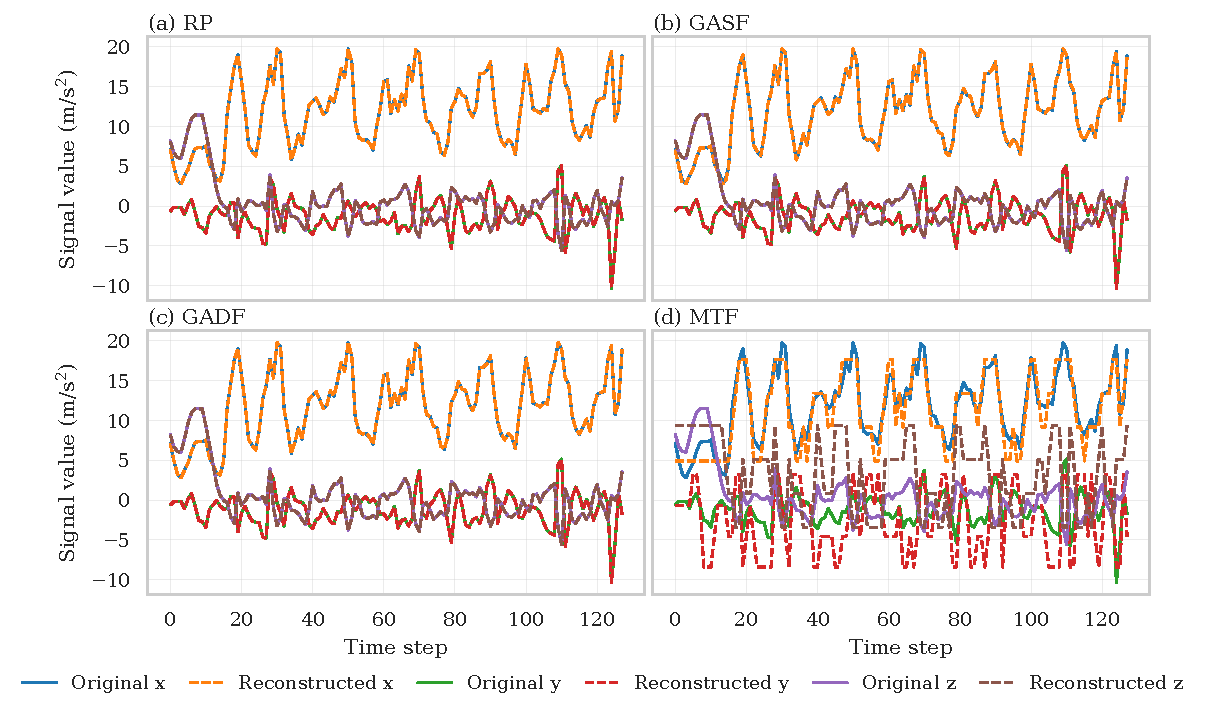
\includegraphics[width=\textwidth]{images/reconstruction_grid.pdf}
\caption{Qualitative reconstruction of one triaxial WISDM walking window from its stored image representation. Original and reconstructed signals are overlaid for each of the four methods, on shared axes.}\label{fig:qualitative_main}
\end{figure}

\subsection{Reconstruction fidelity}

Table~\ref{tab:pointwise_pooled} reports pooled fidelity over all 8,172 windows. Each deterministic decoder scores every window exactly once, so these values are identical under the trial-out and subject-out partitions.

\begin{table}[H]
\centering
\caption{Pooled reconstruction fidelity over 8,172 windows, each entry the per-window metric averaged over the three axes and then over windows (mean$\pm$std across windows). MAE is in m/s\(^2\); NMAE and \(\Delta\)-NMAE are dimensionless and given in units of \(10^{-3}\); Pearson is dimensionless. MSE, NRMSE, spectral energy and band-mass errors, and the per-axis breakdown are in the Supplementary Material. Pearson is given as the pooled mean alone; its across-window dispersion is at most \(1.4\times10^{-4}\) for the near-original trio and \(0.49\) for MTF.}\label{tab:pointwise_pooled}
\footnotesize
\setlength{\tabcolsep}{3pt}
\begin{tabular}{lcccccc}
\toprule
Method & MAE & NMAE & \(\Delta\)-NMAE & Pearson & PSD shape & \(\Delta f\) (Hz) \\
\midrule
RP   & \(0.0142\pm0.0156\) & \(1.0\pm0.7\)     & \(1.2\pm0.8\)   & 0.99998 & \(0.0040\pm0.0022\) & \(0.007\pm0.107\) \\
GASF & \(0.0205\pm0.0199\) & \(1.5\pm0.6\)     & \(2.1\pm0.7\)   & 0.99988 & \(0.0071\pm0.0051\) & \(0.007\pm0.085\) \\
GADF & \(0.0157\pm0.0167\) & \(1.3\pm0.5\)     & \(0.9\pm0.3\)   & 0.99999 & \(0.0026\pm0.0019\) & \(0.005\pm0.081\) \\
MTF  & \(3.94\pm4.25\)     & \(278\pm80\)      & \(202\pm69\)    & 0.014   & \(0.362\pm0.181\)   & \(0.573\pm1.111\) \\
\bottomrule
\end{tabular}
\end{table}

RP, GASF, and GADF sit near the clean 8-bit round-trip floor and preserve both spectral shape and dominant frequency on average, whereas MTF is orders of magnitude less accurate pointwise and loses the spectrum with it. The nonzero standard deviations make these aggregate statements rather than per-window bounds.

Paired window-level Wilcoxon tests distinguish every encoder pair after Holm correction. The practically important effect is the separation from MTF: RP, GASF, and GADF each show a large effect (\(|r|=0.866\)) against it. Differences within the near-original trio are small in absolute units despite statistical detection at \(N=8{,}172\). Repeating the test on 51 subject means preserves the MTF separation and the modest ordering within the trio --- per-subject mean MAE 0.0137 for RP, 0.0148 for GADF, and 0.0199 for GASF, with RP over GADF at \(p=8.6\times10^{-5}\) after Holm correction over the six encoder pairs --- showing that these findings are not produced solely by window-level pseudoreplication. Per-fold and per-axis breakdowns, and the full per-classifier subject-clustered equivalence under both protocols, are in the Supplementary Material.

\subsection{Robustness to image perturbation}\label{sec:results_robustness}

The implementation follows the local-stability protocol defined above. The activity-balanced sample contains 30 windows per class and covers 39 of the 51 subjects. The self-consistency objects are the newly decoded clean reconstruction \(\hat x^{(0)}_{m,w}\) and its cached pipeline counterpart \(\hat x^{\mathrm{cache}}_{m,w}\); all four methods passed the per-window gate.

Table~\ref{tab:robustness} and Figure~\ref{fig:robustness_curves} show increasing error for the three near-original decoders, but no catastrophic failure within the tested range: at \(\sigma=16\) (about \(6\%\) of the intensity range), their mean NMAE remains below \(0.07\). RP has the lowest descriptive mean at every nonzero level, \(0.033\) at \(\sigma=16\). The second position depends on the level: GADF lies between RP and GASF for \(\sigma\le8\), whereas at \(\sigma=16\) GASF (\(0.064\)) overtakes GADF (\(0.065\)). This experiment was not designed as a pairwise superiority test, so we do not infer a population-level robustness ranking from those means alone. MTF stays near \(0.27\) across the curve because its representative reconstruction is already dominated by intrinsic quantisation loss. Subject-cluster intervals and cycle residuals are reported in the Supplementary Material. These results quantify local stability only; they do not cover the coherent structural defects of generated images.

\begin{table}[H]
\centering
\caption{Controlled local-stability test: NMAE, in units of \(10^{-3}\), under zero-mean Gaussian pixel noise (standard deviation \(\sigma\), out of 255). Values are mean$\pm$standard deviation across 150 activity-balanced, subject-spread windows after averaging two independent draws per nonzero level. Subject-cluster 95\% intervals are in the Supplementary Material.}\label{tab:robustness}
\footnotesize
\setlength{\tabcolsep}{3pt}
\begin{tabular}{lccccc}
\toprule
Method & \(\sigma=0\) & \(\sigma=2\) & \(\sigma=4\) & \(\sigma=8\) & \(\sigma=16\) \\
\midrule
RP   & $1.1\pm1.4$     & $4.4\pm3.5$     & $8.2\pm5.0$     & $16.0\pm8.3$    & $32.7\pm13.3$   \\
GASF & $1.6\pm0.9$     & $14.0\pm5.3$    & $21.7\pm5.9$    & $36.7\pm6.9$    & $63.6\pm10.1$   \\
GADF & $1.3\pm0.6$     & $7.8\pm2.2$     & $15.4\pm3.7$    & $32.8\pm8.8$    & $64.9\pm12.6$   \\
MTF  & $270.1\pm81.4$  & $272.2\pm84.5$  & $273.0\pm83.0$  & $273.0\pm82.4$  & $270.0\pm83.1$  \\
\bottomrule
\end{tabular}
\end{table}

\begin{figure}[H]
\centering
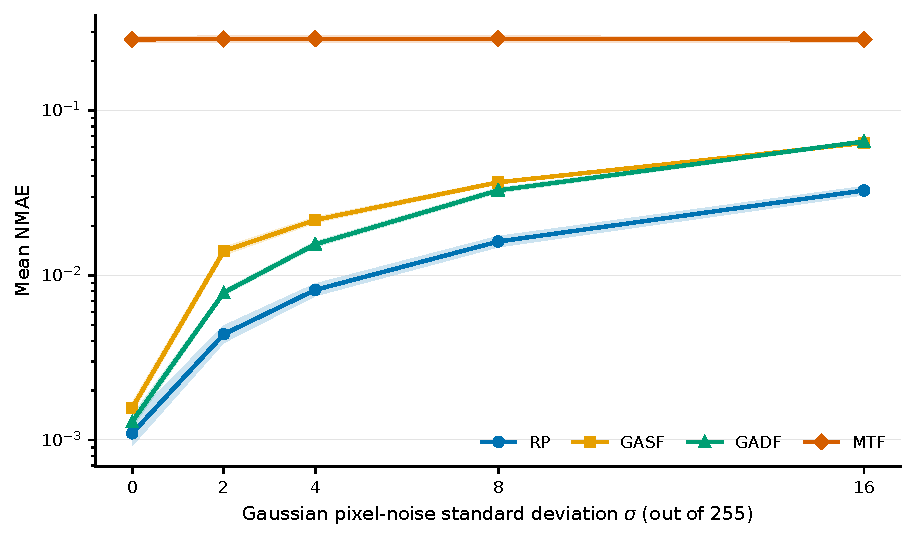
\includegraphics[width=\textwidth]{images/robustness_curves.pdf}
\caption{Reconstruction stability under Gaussian pixel perturbation. Mean NMAE over the 150 activity-balanced WISDM windows as a function of the pixel-noise standard deviation \(\sigma\), out of 255. Shaded regions are subject-cluster 95\% bootstrap intervals and the vertical axis is logarithmic.}\label{fig:robustness_curves}
\end{figure}

Decoding the same 150 windows from the native floating-point operators separates the error sources. RP, GASF, and GADF reconstruct to numerical precision that way, with mean NMAE below \(10^{-16}\), so their remaining clean error is attributable to 8-bit storage; MTF is already lossy before storage. The full decomposition across the native operator, the clean round trip, and perturbation at \(\sigma=8\) is in the Supplementary Material.

\subsection{Downstream classification}\label{sec:subject_out_results}

Table~\ref{tab:subject_out_acc} is the main classification result, under the primary grouped subject-out protocol. RP, GASF, and GADF track the original signal on every classifier, while MTF degrades all of them. The corresponding within-population trial-out accuracies and all six classifiers are reported in the Supplementary Material; both protocols preserve this grouping, although the near-original methods exchange tiny descriptive positions across classifiers.

\begin{table}[H]
\centering
\caption{Grouped subject-out three-fold accuracy (primary protocol) for three representative classifiers spanning the families (convolutional, recurrent, classical). Accuracies are rounded to three decimals; the sub-$0.001$ per-method differences are quantified per subject in Table~\ref{tab:equivalence_ci}. All six classifiers and the trial-out comparison are in the Supplementary Material.}\label{tab:subject_out_acc}
\begin{tabular}{lccccc}
\toprule
Classifier & Original & RP & GASF & GADF & MTF \\
\midrule
CNN & 0.796 & 0.796 & 0.796 & 0.796 & 0.686 \\
GRU & 0.811 & 0.811 & 0.811 & 0.811 & 0.702 \\
RF  & 0.786 & 0.786 & 0.787 & 0.787 & 0.689 \\
\bottomrule
\end{tabular}
\end{table}

McNemar difference tests are secondary because failure to reject a difference does not establish equivalence. The primary result is Table~\ref{tab:equivalence_ci}: each classifier-specific simultaneous interval lies within \(\pm0.01\) for RP, GASF, and GADF, even when complete subjects are held out. For each method the table reports the single simultaneous interval whose endpoint lies closest to the margin, with the classifier it belongs to; every such worst-case interval remains inside \(\pm0.01\). Figure~\ref{fig:equivalence_forest} shows all 24 individual intervals, which the Supplementary Material also tabulates. Holm-adjusted TOST gives the same method-level verdict. MTF is equivalent to none: its mean per-subject accuracy deficit ranges from 0.05 to 0.11 under subject-out.

\begin{table}[H]
\centering
\caption{Subject-level classification equivalence under grouped subject-out validation. The primary family comprises 18 simultaneous subject-cluster bootstrap intervals (six classifiers by RP/GASF/GADF); the six MTF negative-control comparisons form a separate family (51 subjects, \(10^4\) joint resamples per family). For each method, ``most boundary-near'' is the single simultaneous interval whose endpoint lies closest to the equivalence margin, with the classifier it comes from.}\label{tab:equivalence_ci}
\small
\setlength{\tabcolsep}{4pt}
\begin{tabular}{lccccc}
\toprule
 & & \multicolumn{2}{c}{Boundary-near 95\% CI} & \multicolumn{2}{c}{Equivalent} \\
\cmidrule(lr){3-4}\cmidrule(lr){5-6}
Method & Mean \(\Delta\)acc range & Interval & Classifier & \(\pm0.01\) & \(\pm0.02\) \\
\midrule
RP   & \([-0.0004,+0.0006]\) & \([-0.0016,+0.0027]\) & RF  & 6/6 & 6/6 \\
GASF & \([-0.0006,+0.0003]\) & \([-0.0027,+0.0016]\) & RF  & 6/6 & 6/6 \\
GADF & \([-0.0005,+0.0008]\) & \([-0.0013,+0.0030]\) & SVM & 6/6 & 6/6 \\
MTF  & \([+0.0474,+0.1144]\) & \([+0.0212,+0.0736]\) & KNN & 0/6 & 0/6 \\
\bottomrule
\end{tabular}
\end{table}

\begin{figure}[H]
\centering
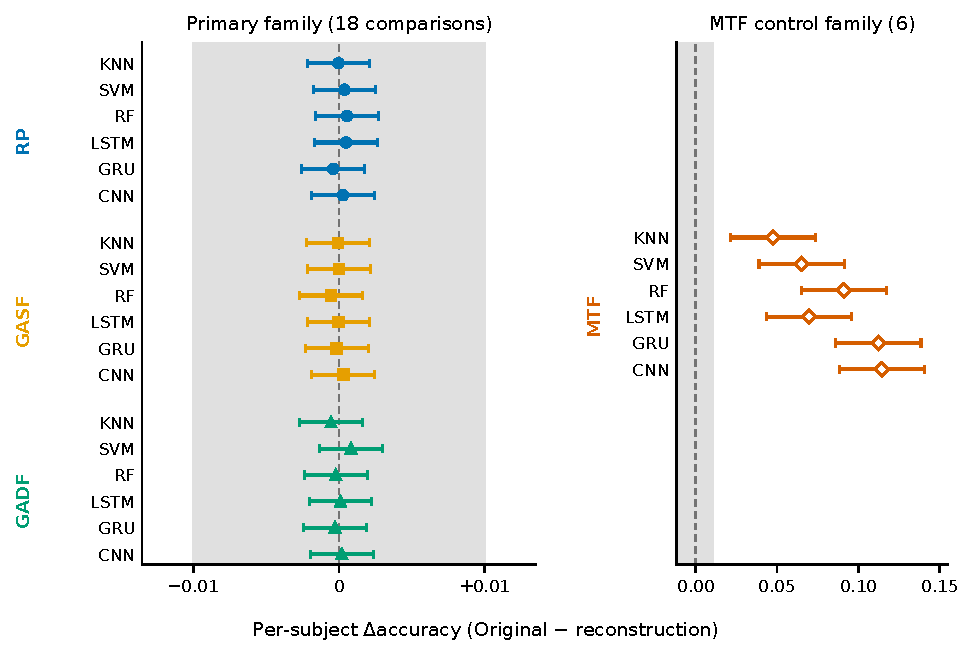
\includegraphics[width=\textwidth]{images/equivalence_forest.pdf}
\caption{Subject-level classification equivalence under grouped subject-out validation. Each row is one classifier--method comparison: markers show the mean per-subject accuracy difference over the 51 subjects, horizontal bars the simultaneous 95\% subject-cluster bootstrap interval, filled when that interval lies wholly inside the shaded \(\pm0.01\) equivalence margin and hollow otherwise. The two panels use different horizontal scales.}\label{fig:equivalence_forest}
\end{figure}

\subsection{Decoder-mechanism ablations}\label{sec:decoder_ablation}

These ablations probe the mechanisms behind the headline RP and GADF decoders; none of them was selected on an outer-fold test set. Table~\ref{tab:ablation_summary} reports the decision-changing comparisons, with the sample and the controlled factors for each row stated in the Supplementary Material.

The orientation step is isolated separately, on 150 activity-balanced windows with the same metadata-free inversion in both arms, and yields three results. The closed form is exact on the unquantised operator, where the 720-angle grid retains its discretisation error. It stays slightly ahead after 8-bit storage, until pixel noise comes to dominate the orientation term. And it more than halves the measured decoding time; among its four candidates it never mis-selects in floating point and does so for 2 of 450 axis-series after clean 8-bit storage. The values behind those statements, together with the GADF pivot sweep, the controlled MTF decoder comparison, the bin-count sensitivity analysis, and the historical regression against the earlier production snapshot, are in the Supplementary Material.

\begin{table}[H]
\centering
\caption{Compact decoder-ablation summary. MAE is in physical units (m/s\(^2\)); the sample and controlled factors for each row are detailed in the Supplementary Material.}\label{tab:ablation_summary}
\small
\resizebox{\textwidth}{!}{%
\begin{tabular}{llll}
\toprule
Method & Used variant (MAE) & Degraded alternative (MAE) & Interpretation \\
\midrule
RP geometry & diagonal-centred + signed (0.011) & signal-range inversion (1.691) & same 100 windows; closed form in both 2-D arms \\
GADF & five pivots (0.0158) & one pivot (0.0353) & averaging suppresses PNG noise \\
MTF & Fiedler ordering (3.95) & cosine pivot (5.39) & spectral ordering helps; still quantisation-lossy \\
\bottomrule
\end{tabular}}
\end{table}

\section{Discussion}\label{sec:discussion}

\subsection{Interpretation of the comparison}\label{sec:disc_pointwise}

The fidelity and utility blocks support one consistent division. RP, GASF, and GADF reconstruct near the clean 8-bit round-trip floor, preserve spectral shape on average, and remain equivalent to the raw signal for original-trained classification under both protocols, whereas MTF is worse on every block. Classification alone would not have established this: a coarse representation can retain class information while losing amplitude, and only the pointwise and spectral metrics show that the three leading methods recover the signal under their stated contracts while MTF preserves a quantile-transition summary.

The small ordering within that trio should not obscure the division. RP attains the lowest mean MAE and NMAE, and GADF the highest correlation, the lowest local-change error and, on the tail-sensitive MSE, the lowest pooled error as well (Supplementary Material). These differences are tiny against the gap to MTF and produce no detectable classification separation, so the practical choice rests on the decoder contract rather than on fidelity: GASF is the simplest faithful baseline, GADF recovers directional differences under a restricted branch, and RP preserves recurrence geometry at the cost of an MDS embedding. Holding out complete subjects lowers absolute accuracy without altering the grouping, and the simultaneous subject-cluster intervals turn a non-significant difference into a positive, margin-relative equivalence statement.

\subsection{Relationship between signed RP and GADF}\label{sec:disc_structural}

Signed RP and GADF are not equivalent matrices, but both encode directional pairwise differences. For slowly varying local increments, let \(\bar x_{ij}\) denote a common local expansion amplitude between the restricted-normalisation samples \(\bar x_i\) and \(\bar x_j\). Then
\[
R_{ij}\approx \sigma(i,j)\sqrt2\,|x_i-x_j|,
\qquad
G^{\mathrm D}_{ij}\approx
\frac{\bar x_j-\bar x_i}{\sqrt{1-\bar x_{ij}^2}}.
\]
GADF is intrinsically antisymmetric because its sign follows from \(\sin(\phi_i-\phi_j)\); the Lu--Tong RP applies an external directional sign and need not be exactly antisymmetric. This analogy explains their visual proximity without implying a shared inverse or formal information equivalence. The full operator derivation and null-corrected regional-overlap diagnostic are provided in the Supplementary Material.

\subsection{Limitations and scope}\label{sec:disc_scope}
\begin{itemize}
\item \textbf{Controlled inputs and generative validity.} Every image is the deterministic output of a known encoder. The repeated Gaussian-noise experiment measures only local pixel stability; it does not cover structural invalidity, occlusion, missing anchors, non-Euclidean RP matrices, or genuinely generated images, so no augmentation benefit is demonstrated.
\item \textbf{Decoder contracts and calibration.} All four decoders return an image-derived normalised trajectory with no method-specific per-window metadata, but returning to physical units requires the common per-axis calibration \((x_{\min},x_{\max})\) equally for every method. Because the WISDM full-scale range is undocumented this uses each window's observed extremes; in a generative setting, where no source window exists, it would have to come from device metadata or be estimated. GASF assumes a fixed branch, and GADF requires \(\alpha<1/\sqrt2\), a consistent sign convention, and a detectable boundary that near-constant or heavily perturbed images may not provide. The near-original tier is measured after an 8-bit round trip, and other storage formats may move that floor.
\item \textbf{Statistical and external validity.} Pooled window tests understate intra-subject dependence; the primary intervals resample whole subjects and control the 18-comparison family, with MTF handled separately, and equivalence remains relative to the chosen margin. Only 8,032 of the 8,172 windows are distinct as (window, subject, activity) triples, the remaining 140 repeating an identical earlier window of the source stream, so pooled window-level tests slightly overstate the number of independent observations. Results cover one smartwatch accelerometer dataset, five activities, 51 subjects, 20\,Hz sampling, and \(N=128\) windows.
\item \textbf{Decoder cost.} The RP decoder remains dominated by the classical-MDS eigendecomposition, \(O(N^3)\) per axis, which is inexpensive at \(N=128\) but would require an approximate or incremental embedding for long windows, with untested effect on fidelity. GASF, GADF, and MTF decode in \(O(N^2)\).
\end{itemize}

\section{Conclusion}\label{sec:conclusion}

This work establishes when an image-based time-series representation can be treated as a reversible signal representation rather than only as a visual feature map. Two decoders make that account operational. For the continuous signed adjacent-state RP, the zero-valued diagonal removes the need to store the per-window operator range, while two-dimensional classical MDS, overlap alignment, and closed-form orientation with signed selection recover the normalised waveform from the image alone. For GADF, restricting the angular branch makes the relative angles uniquely recoverable, an image-derived boundary anchor restores their global offset, and multi-pivot averaging reduces quantisation error. Neither requires method-specific per-window metadata. Against them, the established GASF diagonal inverse is the baseline and the Fiedler-ordered MTF output marks the limit of reconstruction, since quantile assignment is many-to-one.

On 8,172 WISDM windows this yields a clear information hierarchy. RP, GASF, and GADF form a near-lossless tier with mean MAEs of 0.0142, 0.0205, and 0.0157\,m/s$^2$; all three are exact at the native floating-operator level, so their clean residual error is attributable to 8-bit storage alone, and the fidelity survives the downstream task, with all 18 RP/GASF/GADF accuracy differences inside a one-percentage-point equivalence region across six classifiers and complete held-out subjects. MTF stays substantially lossy throughout, which is why downstream usefulness alone should not be read as invertibility. The conclusions hold for images produced by known encoders: the perturbation experiment establishes local stability, not validity under arbitrary image defects, and physical-unit recovery still requires the shared amplitude calibration. Evaluating structurally imperfect and genuinely generated encoding images is the next step, and the decoder contracts established here are what it needs to start from.

\section*{Credit authorship contribution statement}

\noindent
\textbf{Adriano García-Giralda Milena:}
Conceptualization, Methodology, Software, Formal analysis,
Investigation, Data curation, Validation, Visualization,
Writing -- original draft, Writing -- review \& editing.

\noindent
\textbf{Francisco García Moreno:}
Conceptualization, Methodology, Supervision,
Writing -- review \& editing.

\noindent
\textbf{José Antonio Jiménez Madrid:}
Methodology, Formal analysis,
Writing -- review \& editing.

\noindent
\textbf{María Bermúdez Edo:}
Supervision, Writing -- review \& editing.
\section*{Funding}

% Declare the funding received.
% If none was received:
This research did not receive any specific grant
from funding agencies in the public, commercial,
or not-for-profit sectors.


\section*{Data availability}

The WISDM Smartphone and Smartwatch Activity and
Biometrics Dataset used in this study is publicly
available through the UCI Machine Learning Repository
(\url{https://doi.org/10.24432/C5HK59}).

The source code and supporting materials associated
with this research are hosted on GitHub:
\url{https://github.com/adrianoggm/TFG-Tratamiento-de-Series-Temporales}.

\section*{Declaration of generative AI and AI-assisted
technologies in the manuscript preparation process}

During the preparation of this work, the authors used
ChatGPT (OpenAI) to assist with manuscript structuring,
scientific writing, language refinement, and improving
the clarity of technical explanations. All AI-assisted
content was critically reviewed, verified, and revised
by the authors, who take full responsibility for the
accuracy, originality, and integrity of the final
manuscript.

{\small
\begin{thebibliography}{99}
\setlength{\itemsep}{0pt}
\setlength{\parskip}{0pt}
\raggedright

\bibitem{wang2015encoding}
Zhiguang Wang and Tim Oates. ``Imaging time-series to improve classification and imputation''. In \textit{Proceedings of the 24th International Joint Conference on Artificial Intelligence (IJCAI)}, pp. 3939--3945, 2015.

\bibitem{wang2015encoding2}
Zhiguang Wang and Tim Oates. ``Encoding time series as images for visual inspection and classification using tiled convolutional neural networks''. In \textit{Workshops at the Twenty-Ninth AAAI Conference on Artificial Intelligence}, 2015.

\bibitem{huang2023tsdigan}
Tongge Huang, Pranamesh Chakraborty, and Anuj Sharma. ``Deep convolutional generative adversarial networks for traffic data imputation encoding time series as images''. \textit{International Journal of Transportation Science and Technology}, vol. 12, no. 1, pp. 1--18, 2023. doi: \url{https://doi.org/10.1016/j.ijtst.2021.10.007}.

\bibitem{hellermann2026imagegan}
Justin Hellermann and Stefan Lessmann. ``Leveraging image-based generative adversarial networks for time series generation''. \textit{International Journal of Forecasting}, vol. 42, no. 2, pp. 616--639, 2026. doi: \url{https://doi.org/10.1016/j.ijforecast.2025.09.004}.

\bibitem{eckmann1987recurrence}
Jean-Pierre Eckmann, S. Oliffson Kamphorst, and David Ruelle. ``Recurrence plots of dynamical systems''. \textit{Europhysics Letters}, vol. 4, no. 9, pp. 973--977, 1987. doi: \url{https://doi.org/10.1209/0295-5075/4/9/004}.

\bibitem{marwan2007recurrence}
Norbert Marwan, M. Carmen Romano, Marco Thiel, and Jürgen Kurths. ``Recurrence plots for the analysis of complex systems''. \textit{Physics Reports}, vol. 438, no. 5--6, pp. 237--329, 2007. doi: \url{https://doi.org/10.1016/j.physrep.2006.11.001}.

\bibitem{ahmad2021inertial}
Zeeshan Ahmad and Naimul Khan. ``Inertial sensor data to image encoding for human action recognition''. \textit{IEEE Sensors Journal}, vol. 21, no. 9, pp. 10978--10988, 2021. doi: \url{https://doi.org/10.1109/JSEN.2021.3062261}.

\bibitem{ma2024anomaly}
Jidong Ma and Hairu Wang. ``Anomaly detection in sensor data via encoding time series into images''. \textit{Journal of King Saud University -- Computer and Information Sciences}, vol. 36, no. 10, article 102232, 2024. doi: \url{https://doi.org/10.1016/j.jksuci.2024.102232}.

\bibitem{huamin2020reconstruction}
Huamin Tao, Qiuqun Deng, and Shanzhu Xiao. ``Reconstruction of time series with missing value using 2D representation-based denoising autoencoder''. \textit{Journal of Systems Engineering and Electronics}, vol. 31, no. 6, pp. 1087--1096, 2020. doi: \url{https://doi.org/10.23919/JSEE.2020.000081}.

\bibitem{takens1981detecting}
Floris Takens. ``Detecting strange attractors in turbulence''. In \textit{Dynamical Systems and Turbulence, Warwick 1980}, Lecture Notes in Mathematics, vol. 898, pp. 366--381, Springer, 1981. doi: \url{https://doi.org/10.1007/BFb0091924}.

\bibitem{lu2019robust}
Jianjie Lu and Kai-Yu Tong. ``Robust single accelerometer-based activity recognition using modified recurrence plot''. \textit{IEEE Sensors Journal}, vol. 19, no. 15, pp. 6317--6324, 2019. doi: \url{https://doi.org/10.1109/JSEN.2019.2911204}.

\bibitem{hirata2008reproduction}
Yoshito Hirata, Shunsuke Horai, and Kazuyuki Aihara. ``Reproduction of distance matrices and original time series from recurrence plots and their applications''. \textit{The European Physical Journal Special Topics}, vol. 164, no. 1, pp. 13--22, 2008. doi: \url{https://doi.org/10.1140/epjst/e2008-00830-8}.

\bibitem{sipers2011unique}
Aloys Sipers, Paul J. A. Borm, and Ralf L. M. Peeters. ``On the unique reconstruction of a signal from its unthresholded recurrence plot''. \textit{Physics Letters A}, vol. 375, no. 24, pp. 2309--2321, 2011. doi: \url{https://doi.org/10.1016/j.physleta.2011.04.040}.

\bibitem{sipers2017robust}
Aloys Sipers, Paul J. A. Borm, and Ralf L. M. Peeters. ``Robust reconstruction of a signal from its unthresholded recurrence plot subject to disturbances''. \textit{Physics Letters A}, vol. 381, no. 6, pp. 604--615, 2017. doi: \url{https://doi.org/10.1016/j.physleta.2016.12.028}.

\bibitem{Torgerson1952}
Warren S. Torgerson. ``Multidimensional scaling: I. Theory and method''. \textit{Psychometrika}, vol. 17, no. 4, pp. 401--419, 1952. doi: \url{https://doi.org/10.1007/BF02288916}.

\bibitem{Atkins1998}
Jonathan E. Atkins, Erik G. Boman, and Bruce Hendrickson. ``A spectral algorithm for seriation and the consecutive ones problem''. \textit{SIAM Journal on Computing}, vol. 28, no. 1, pp. 297--310, 1998. doi: \url{https://doi.org/10.1137/S0097539795285771}.

\bibitem{misc_wisdm_smartphone_and_smartwatch_activity_and_biometrics_dataset__507}
Gary M. Weiss. ``WISDM Smartphone and Smartwatch Activity and Biometrics Dataset''. \textit{UCI Machine Learning Repository}, 2019. doi: \url{https://doi.org/10.24432/C5HK59}.

\bibitem{Welch1967}
Peter D. Welch. ``The use of fast Fourier transform for the estimation of power spectra: A method based on time averaging over short, modified periodograms''. \textit{IEEE Transactions on Audio and Electroacoustics}, vol. 15, no. 2, pp. 70--73, 1967. doi: \url{https://doi.org/10.1109/TAU.1967.1161901}.

\bibitem{Wilcoxon1945}
Frank Wilcoxon. ``Individual comparisons by ranking methods''. \textit{Biometrics Bulletin}, vol. 1, no. 6, pp. 80--83, 1945. doi: \url{https://doi.org/10.2307/3001968}.

\bibitem{McNemar1947}
Quinn McNemar. ``Note on the sampling error of the difference between correlated proportions or percentages''. \textit{Psychometrika}, vol. 12, no. 2, pp. 153--157, 1947. doi: \url{https://doi.org/10.1007/BF02295996}.

\bibitem{DavisonHinkley1997}
Anthony C. Davison and David V. Hinkley. \textit{Bootstrap Methods and Their Application}. Cambridge University Press, 1997.

\bibitem{Hall1987}
Peter Hall. ``On the bootstrap and likelihood-based confidence regions''. \textit{Biometrika}, vol. 74, no. 3, pp. 481--493, 1987. doi: \url{https://doi.org/10.1093/biomet/74.3.481}.

\bibitem{Lakens2017}
Daniël Lakens. ``Equivalence tests: A practical primer for t tests, correlations, and meta-analyses''. \textit{Social Psychological and Personality Science}, vol. 8, no. 4, pp. 355--362, 2017. doi: \url{https://doi.org/10.1177/1948550617697177}.

\bibitem{Schuirmann1987}
Donald J. Schuirmann. ``A comparison of the two one-sided tests procedure and the power approach for assessing the equivalence of average bioavailability''. \textit{Journal of Pharmacokinetics and Biopharmaceutics}, vol. 15, no. 6, pp. 657--680, 1987. doi: \url{https://doi.org/10.1007/BF01068419}.

\bibitem{Holm1979}
Sture Holm. ``A simple sequentially rejective multiple test procedure''. \textit{Scandinavian Journal of Statistics}, vol. 6, no. 2, pp. 65--70, 1979.
\end{thebibliography}
}
\end{document}
